\documentclass[a4paper,12pt]{article}
\usepackage{parskip}
\usepackage{graphicx}
\usepackage{float}
\usepackage{enumerate}

%Note - the tilde (~) adds a non-breaking space. You can use a normal space if you like, but the space may appear at the end of the line which would look ugly

\begin{document}
\section{Introduction}
Many things in \LaTeX\ can be referenced, such as sections, subsections, subsubsections, tables, figures, individual items in a list, equations etc. The commands used are the same, no matter what you are referencing. These are:

\verb|\label{marker}| - this is used to mark the thing you are referencing

\verb|\ref{marker}| - this returns the reference to the thing you are marking

\verb|\pageref{marker}| - this returns the page number of the thing you are marking

\subsection{Conventions}
\label{subsec:convention}

It is common among \LaTeX\ users to start the marker with a few specific letters to indicate what it is they are referencing. E.g.\ an example marker for a figure would be \verb|fig:exampleImage|, but for a section, it would be \verb|sec:exampleSection|. Table~\ref{tab:convention} outlines the convention used:

\begin{table}[H]
  \centering
  \begin{tabular}{|l|l|}
    \hline
    {\bf ch:}     & chapter              \\ \hline
    {\bf sec:}    & section              \\ \hline
    {\bf subsec:} & subsection           \\ \hline
    {\bf fig:}    & figure               \\ \hline
    {\bf tab:}    & table                \\ \hline
    {\bf eq:}     & equation             \\ \hline
    {\bf lst:}    & code listing         \\ \hline
    {\bf itm:}    & enumerated list item \\ \hline
    {\bf alg:}    & algorithm            \\ \hline
    {\bf app:}    & appendix subsection  \\ \hline
  \end{tabular}
  \caption{Conventions used}
  \label{tab:convention}
\end{table}

\section{Examples}

\subsection{Figures}
To reference a picture, add the \verb|\label| command \emph{after} the caption line:
\begin{figure}[H]
  \centering
  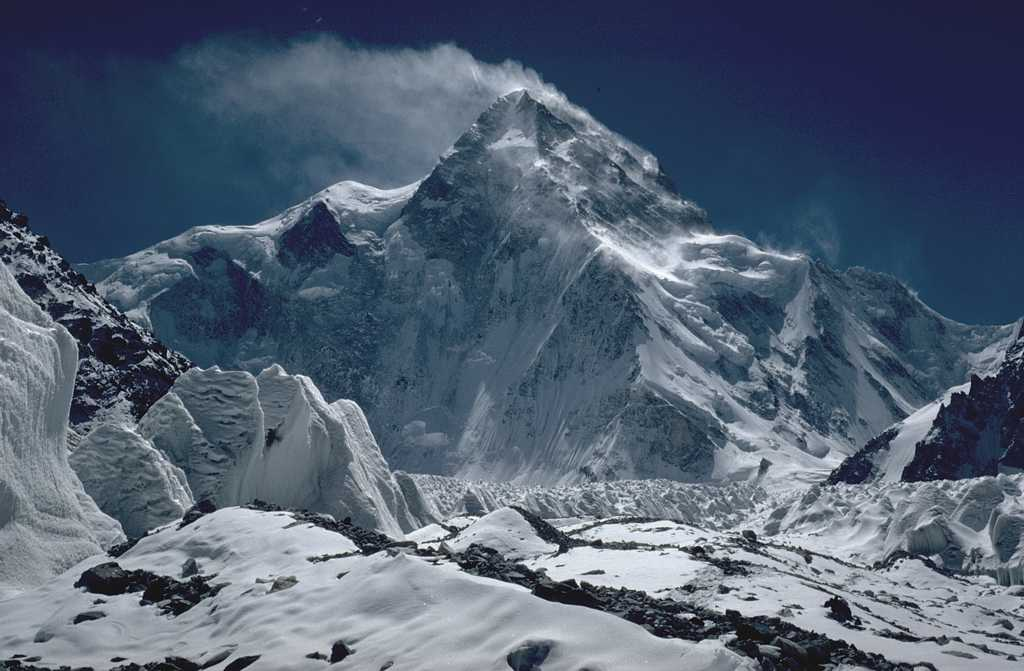
\includegraphics[width=0.9\textwidth]{k2.jpg}
  \caption{The K2 mountain in Baltistan}
  \label{fig:k2}
\end{figure}

Figure~\ref{fig:k2} on page~\pageref{fig:k2} shows a picture of the K2 mountain.

\subsection{Sections}
We can also reference a subsection by placing a \verb|\label| command right after the subsection line, e.g.\ we talked about conventions in section~\ref{subsec:convention} on page~\pageref{subsec:convention}.

\subsection{Lists}
\begin{enumerate}
  \item Dog
    \begin{enumerate}
      \item Labrador
        \begin{enumerate}
          \item English Labrador
            \label{itm:englishLab}
          \item American Labrador
        \end{enumerate}
      \item Alsation
      \item Pug
    \end{enumerate}
  \item Cat
    \begin{itemize}
      \item Persian
        \label{itm:persian}
      \item British shorthair
      \item Siamese
      \item Bengal
    \end{itemize}
\end{enumerate}

As we can see from item \ref{itm:englishLab}, the English Labrador is a type of dog.

Also, as we can see from item \ref{itm:persian}, there is a type of cat which is called a Persian cat.

\section{Final warning}
Often in \LaTeX, you need to compile a document more than once for it to compile properly. If you put in new references, then compile your document, you will come up with a warning such as:

\begin{verbatim}
Reference `itm:englishLab' on page 3 undefined on input line 82.
\end{verbatim}

Just compile the document again, and the warning should go away. If it doesn't, make sure you have written the reference down correctly and that the \verb|\label| command is there. In the case of figures and tables, ensure that the \verb|\label| command is after the \verb|\caption| command.

\end{document}
